
\documentclass[border=10pt, 12pt]{standalone}
\usepackage[svgnames]{xcolor}
\usepackage{amsmath}
\usepackage{pgfplots}
\pgfplotsset{compat=newest}
\usepackage[sfdefault]{FiraSans}
\usepackage{FiraMono}
\renewcommand*\familydefault{\sfdefault}
\begin{document}
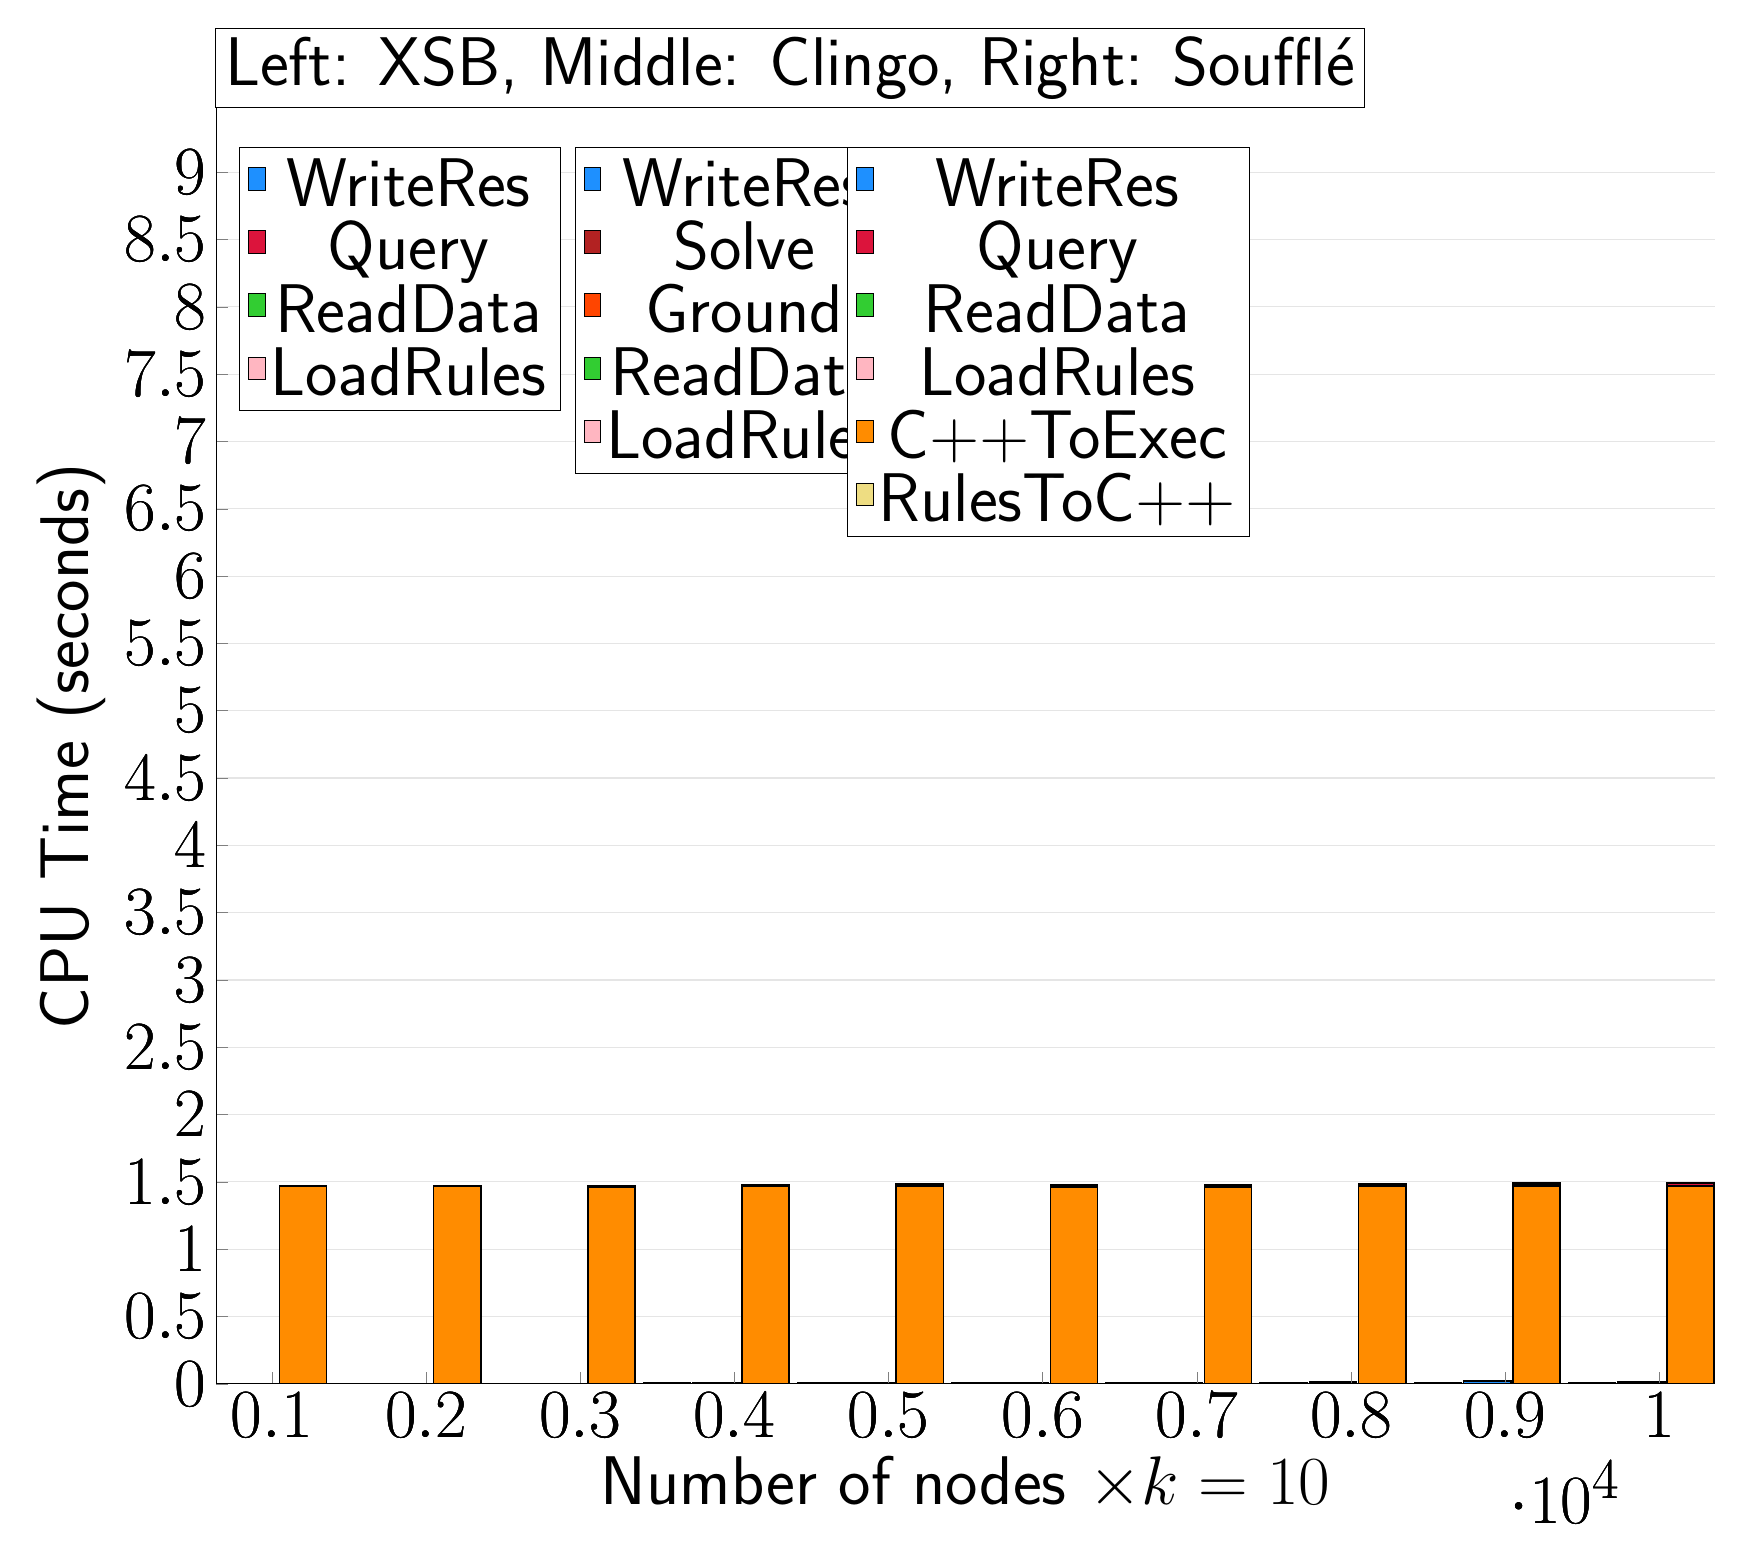
\begin{tikzpicture}
                        \begin{axis}[bar shift=-24.3pt, 
   ybar stacked,
   width=1.7\textwidth,
   bar width=0.6cm,
   ymajorgrids, tick align=inside,
   major grid style={draw=gray!20},
   xtick=data,
   ymin=0, ymax=9.474,
   axis x line*=bottom,
   axis y line*=left,
   enlarge x limits=0.04,
   legend style={
       at={(0.23, 0.97)},
       anchor=north east,
       legend columns=1,
       font=\Huge,
   },
   ylabel={CPU Time (seconds)},
   xlabel={Number of nodes $\times k=10$},
   label style={font=\Huge},
   tick label style={font=\Huge},
]
\addlegendimage{fill=DodgerBlue, draw=black, line width=0.2pt}
\addlegendentry{WriteRes}
\addlegendimage{fill=Crimson, draw=black, line width=0.2pt}
\addlegendentry{Query}
\addlegendimage{fill=LimeGreen, draw=black, line width=0.2pt}
\addlegendentry{ReadData}
\addlegendimage{fill=LightPink, draw=black, line width=0.2pt}
\addlegendentry{LoadRules}
\addplot +[fill=LightPink, draw=black, line width=0.55pt] coordinates {
(1000, 0.0005589999999999992)
(2000, 0.000553)
(3000, 0.0005516000000000003)
(4000, 0.00055)
(5000, 0.0005526000000000002)
(6000, 0.0005528000000000006)
(7000, 0.0005558000000000001)
(8000, 0.0005506000000000003)
(9000, 0.0005524000000000003)
(10000, 0.0005493999999999996)
};
\addplot +[fill=LimeGreen, draw=black, line width=0.55pt] coordinates {
(1000, 0.0002138000000000004)
(2000, 0.0002888000000000006)
(3000, 0.00036679999999999997)
(4000, 0.00044779999999999977)
(5000, 0.0005326)
(6000, 0.0006030000000000002)
(7000, 0.0006699999999999998)
(8000, 0.0007575999999999995)
(9000, 0.0008344000000000001)
(10000, 0.0009287999999999998)
};
\addplot +[fill=Crimson, draw=black, line width=0.55pt] coordinates {
(1000, 7.740000000000004e-05)
(2000, 0.0001361999999999994)
(3000, 0.00019579999999999958)
(4000, 0.00025639999999999984)
(5000, 0.00031680000000000044)
(6000, 0.00037339999999999975)
(7000, 0.00041859999999999977)
(8000, 0.00048659999999999996)
(9000, 0.0005402000000000004)
(10000, 0.0005911999999999998)
};
\addplot +[fill=DodgerBlue, draw=black, line width=0.55pt] coordinates {
(1000, 0.0009069999999999998)
(2000, 0.0017102000000000007)
(3000, 0.0025268000000000005)
(4000, 0.0033268)
(5000, 0.0041264)
(6000, 0.0049462)
(7000, 0.005769999999999999)
(8000, 0.006594600000000001)
(9000, 0.0073402)
(10000, 0.008252)
};
\end{axis}

\begin{axis}[bar shift=-6.5pt, 
   ybar stacked,
   width=1.7\textwidth,
   bar width=0.6cm,
   ymajorgrids, tick align=inside,
   major grid style={draw=none},
   xtick=data,
   ymin=0, ymax=9.474,
   axis x line*=none,
   axis y line*=none,
   enlarge x limits=0.04,
   legend style={
       at={(0.454, 0.97)},
       anchor=north east,
       legend columns=1,
       font=\Huge,
   },
   label style={font=\Huge},
   tick label style={font=\Huge},
]
\addlegendimage{fill=DodgerBlue, draw=black, line width=0.2pt}
\addlegendentry{WriteRes}
\addlegendimage{fill=FireBrick, draw=black, line width=0.2pt}
\addlegendentry{Solve}
\addlegendimage{fill=OrangeRed, draw=black, line width=0.2pt}
\addlegendentry{Ground}
\addlegendimage{fill=LimeGreen, draw=black, line width=0.2pt}
\addlegendentry{ReadData}
\addlegendimage{fill=LightPink, draw=black, line width=0.2pt}
\addlegendentry{LoadRules}
\addplot +[fill=LightPink, draw=black, line width=0.55pt] coordinates {
(1000, 0.0)
(2000, 0.0)
(3000, 0.0)
(4000, 0.0)
(5000, 0.0)
(6000, 0.0)
(7000, 0.0)
(8000, 0.0)
(9000, 0.0)
(10000, 0.0)
};
\addplot +[fill=LimeGreen, draw=black, line width=0.55pt] coordinates {
(1000, 0.0)
(2000, 0.0)
(3000, 0.0)
(4000, 0.0)
(5000, 0.0)
(6000, 0.0)
(7000, 0.0)
(8000, 0.0)
(9000, 0.0)
(10000, 0.0)
};
\addplot +[fill=OrangeRed, draw=black, line width=0.55pt] coordinates {
(1000, 0.0)
(2000, 0.0)
(3000, 0.0)
(4000, 0.0)
(5000, 0.0)
(6000, 0.0)
(7000, 0.0)
(8000, 0.0020000000000000018)
(9000, 0.0040000000000000036)
(10000, 0.006000000000000005)
};
\addplot +[fill=FireBrick, draw=black, line width=0.55pt] coordinates {
(1000, 0.0)
(2000, 0.0)
(3000, 0.0)
(4000, 0.0)
(5000, 0.0)
(6000, 0.0)
(7000, 0.0)
(8000, 0.0020000000000000018)
(9000, 0.0)
(10000, 0.0040000000000000036)
};
\addplot +[fill=DodgerBlue, draw=black, line width=0.55pt] coordinates {
(1000, 0.0)
(2000, 0.0)
(3000, 0.0)
(4000, 0.010000000000000009)
(5000, 0.010000000000000009)
(6000, 0.010000000000000009)
(7000, 0.010000000000000009)
(8000, 0.008000000000000007)
(9000, 0.016000000000000014)
(10000, 0.006000000000000005)
};
\end{axis}

\begin{axis}[bar shift=11.3pt, 
   ybar stacked,
   width=1.7\textwidth,
   bar width=0.6cm,
   ymajorgrids, tick align=inside,
   major grid style={draw=none},
   xtick=data,
   ymin=0, ymax=9.474,
   axis x line*=none,
   axis y line*=none,
   enlarge x limits=0.04,
   legend style={
       at={(0.69, 0.97)},
       anchor=north east,
       legend columns=1,
       font=\Huge,
   },
   label style={font=\Huge},
   tick label style={font=\Huge},
]
\addlegendimage{fill=DodgerBlue, draw=black, line width=0.2pt}
\addlegendentry{WriteRes}
\addlegendimage{fill=Crimson, draw=black, line width=0.2pt}
\addlegendentry{Query}
\addlegendimage{fill=LimeGreen, draw=black, line width=0.2pt}
\addlegendentry{ReadData}
\addlegendimage{fill=LightPink, draw=black, line width=0.2pt}
\addlegendentry{LoadRules}
\addlegendimage{fill=DarkOrange, draw=black, line width=0.2pt}
\addlegendentry{C++ToExec}
\addlegendimage{fill=LightGoldenrod, draw=black, line width=0.2pt}
\addlegendentry{RulesToC++}
\addplot +[fill=LightGoldenrod, draw=black, line width=0.55pt] coordinates {
(1000, 0.0)
(2000, 0.0020000000000000005)
(3000, 0.0)
(4000, 0.0)
(5000, 0.0)
(6000, 0.0020000000000000005)
(7000, 0.0)
(8000, 0.0020000000000000005)
(9000, 0.0020000000000000005)
(10000, 0.0020000000000000005)
};
\addplot +[fill=DarkOrange, draw=black, line width=0.55pt] coordinates {
(1000, 1.466)
(2000, 1.464)
(3000, 1.462)
(4000, 1.468)
(5000, 1.468)
(6000, 1.46)
(7000, 1.46)
(8000, 1.464)
(9000, 1.466)
(10000, 1.466)
};
\addplot +[fill=LightPink, draw=black, line width=0.55pt] coordinates {
(1000, 0.0001462)
(2000, 0.0001584)
(3000, 0.00015920000000000002)
(4000, 0.0001614)
(5000, 0.00016900000000000002)
(6000, 0.00015219999999999999)
(7000, 0.00016480000000000002)
(8000, 0.0001492)
(9000, 0.000161)
(10000, 0.00015460000000000002)
};
\addplot +[fill=LimeGreen, draw=black, line width=0.55pt] coordinates {
(1000, 0.0009195999999999999)
(2000, 0.001249)
(3000, 0.0013978)
(4000, 0.0020926)
(5000, 0.0025614)
(6000, 0.0027114)
(7000, 0.0030868)
(8000, 0.0032672)
(9000, 0.0036792000000000005)
(10000, 0.004202599999999999)
};
\addplot +[fill=Crimson, draw=black, line width=0.55pt] coordinates {
(1000, 0.0022612)
(2000, 0.003946)
(3000, 0.004704)
(4000, 0.007535)
(5000, 0.0088392)
(6000, 0.009482599999999999)
(7000, 0.0115186)
(8000, 0.012756599999999998)
(9000, 0.014303399999999999)
(10000, 0.0159078)
};
\addplot +[fill=DodgerBlue, draw=black, line width=0.55pt] coordinates {
(1000, 0.0012092000000000001)
(2000, 0.0017364000000000001)
(3000, 0.0017752)
(4000, 0.0021376000000000004)
(5000, 0.0029748000000000005)
(6000, 0.002987)
(7000, 0.003474)
(8000, 0.0037274)
(9000, 0.004065)
(10000, 0.0044800000000000005)
};
\end{axis}


\node[anchor=south, draw, fill=white] at (rel axis cs:0.42,1) {\Huge Left: XSB, Middle: Clingo, Right: Soufflé};
\end{tikzpicture}
\end{document}
                    